\section{Pregunta N$^{\circ}$1\qquad Andre Gilmer Santos Felix}

\begin{frame}
    \begin{enumerate}\setcounter{enumi}{0}
        \item

              Calcule la curvatura de la gráfica del polinomio de
              $B_{3,5}\left(t\right)$.
    \end{enumerate}

    \begin{solution}

        \begin{definition}[Polinomio de Bernstein]
            Las funciones base de Bernstein de grado $n$ son
            \begin{equation*}
                \forall t\in\left[0,1\right]
                \forall k\in\left\{0,\dotsc,n\right\}:
                B_{k,n}\left(t\right)=
                \binom{n}{k}
                t^{k}
                \left(1-t\right)^{n-k}
            \end{equation*}.
        \end{definition}

        \begin{theorem}
            Si $B_{k,n}\left(t\right)$, entonces
            \begin{math}
                B^{\prime}_{k,n}\left(t\right)=
                n
                \left[
                    B_{k-1,n-1}\left(t\right)-
                    B_{k,n-1}\left(t\right)-
                    \right]
            \end{math}.
        \end{theorem}

        Sean los polinomios
        \begin{align*}
            B_{3,5}\left(t\right)                & =
            \binom{5}{3}
            t^{3}
            \left(1-t\right)^{5-3}=
            10t^{3}{\left(1-t\right)}^{2}.           \\
            B^{\prime}_{3,5}\left(t\right)       & =
            5
            \left[
                B_{2,4}\left(t\right)-
                B_{3,4}\left(t\right)
                \right]=
            5
            \left[
            \binom{4}{2}t^{2}\left(1-t\right)^{4-2}-
            \binom{4}{3}t^{3}\left(1-t\right)^{4-3}
            \right]=                                 \\
            B^{\prime\prime}_{3,5}\left(t\right) & =
            5\left[B^{\prime}_{2,4}\left(t\right)-B^{\prime}_{3,4}\left(t\right)\right]=
            5\left[
                4\left[B_{2,4}\left(t\right)\right]
                \right].
        \end{align*}

        La curvatura de la gráfica
        \begin{math}
            \left(
            x\left(t\right),
            y\left(t\right)
            \right)=
            \left(
            t,
            B_{3,5}\left(t\right)
            \right)
        \end{math}
        es
        \begin{equation*}
            \kappa\left(t\right)=
            \dfrac{
                y^{\prime\prime}
            }{
                {\left(1+{y^{\prime}}^{2}\right)}^{\frac{3}{2}}
            }=
            \dfrac{1}{1}.
        \end{equation*}
    \end{solution}
\end{frame}

\begin{frame}
    \begin{solution}
        \begin{figure}[ht!]
            \centering
            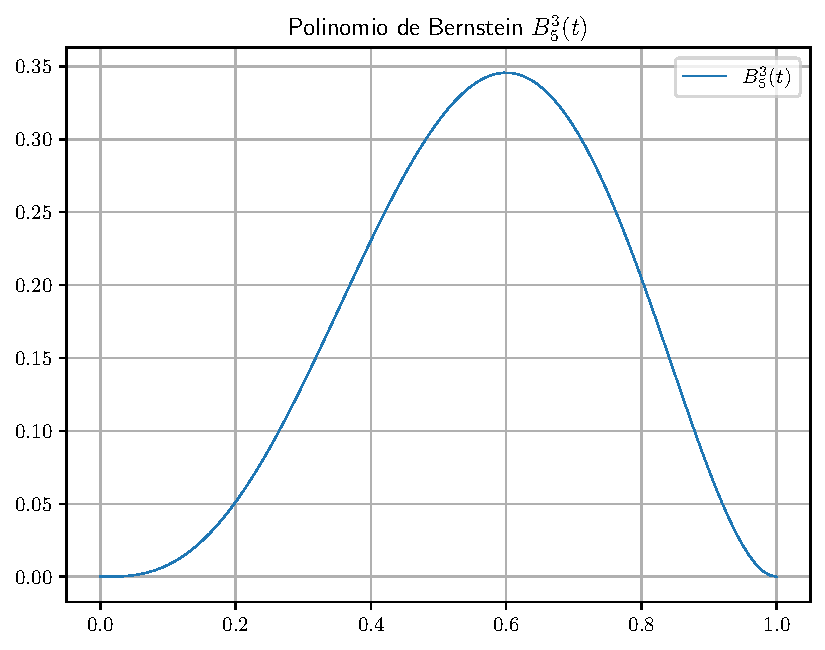
\includegraphics[width=.72\paperwidth]{p1}
        \end{figure}
    \end{solution}
\end{frame}